\clearpage
\chapter{METHODOLOGY}
\section{Research Design and Workflow}
This chapter outlines the computational framework utilized to investigate the aerothermal effects of surface topology on a Hypersonic Inflatable Aerodynamic Decelerator (HIAD). The research workflow follows a sequential numerical analysis approach, moving from parametric geometry generation to high-fidelity Computational Fluid Dynamics (CFD) simulation.

To systematically isolate the effects of the "scalloped" surface geometry, the methodology is designed to compare a baseline rigid sphere-cone against the proposed inflatable architecture under identical hypersonic flight conditions. The workflow is visualized in Figure \ref{fig:flowchart} and consists of four primary stages:

% TODO: INSERT FLOWCHART FIGURE HERE
% Create a block diagram showing: FreeCAD -> 2D Slice -> Meshing -> CFD Setup -> Solution -> Validation
\begin{figure}[H]
    \centering
    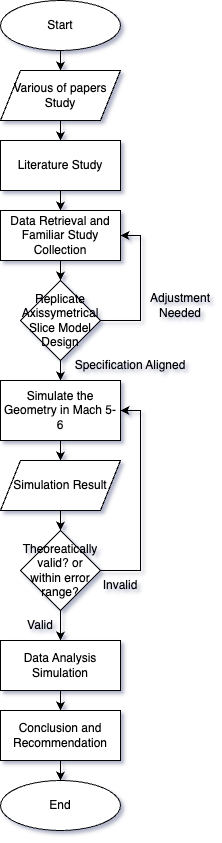
\includegraphics[width=0.273\textwidth]{gambar/flowchart.png}
    \caption{Flowchart of the numerical research methodology.}
    \label{fig:flowchart}
\end{figure}
\par
The process is divided into four primary stages:
\begin{enumerate}
    \item \textbf{Geometric Modeling:} Automated generation of the scalloped (inflatable) and smooth (baseline) profiles using parametric Python scripting in FreeCAD to ensure geometric consistency.
    \item \textbf{Domain Discretization:} Generation of a structured/hybrid mesh with strict near-wall refinement ($y^+ \approx 1$) to resolve the high thermal gradients in the boundary layer.
    \item \textbf{Numerical Configuration:} Setup of the density-based coupled solver, utilizing the SST $k-\omega$ turbulence model and temperature-dependent gas properties (Sutherland’s Law).
    \item \textbf{Validation and Analysis:} Verification of the solution through a grid independence study and validation of the thermal results against theoretical Fay-Riddell correlations.
\end{enumerate}
\section{Geometric Modeling and Computational Domain}

\subsection{Parametric Geometry Generation}
To ensure geometric consistency, the vehicle profiles were generated using a parametric Python script within the FreeCAD environment. The geometric constraints are derived directly from the \textbf{NASA IRVE-3} and \textbf{LOFTID} flight test specifications to ensure the simulation captures flight-representative physics.

\subsection{Vehicle Specifications and Scaling}
The modeling phase targets two specific scales identified in previous NASA research to investigate how vehicle diameter affects the aerothermal environment. As shown in Figure \ref{fig:hiad_comparison}, the research considers the scaling transition from the 4.57m rigid baseline to the 15m large-scale HIAD\cite{dillman2015irve3}.

\begin{figure}[H]
    \centering
    
\includegraphics[width=0.8\textwidth]{Hiad_DesignSpec.png}
    \caption{Geometric comparison between the 15m Inflatable HIAD and the 4.57m Rigid Baseline.}
    \label{fig:hiad_comparison}
\end{figure}

\subsection{Internal Architecture and Scallop Definition}
The "scalloped" OML is modeled based on the 7-toroid stack configuration utilized in the IRVE-3 mission. The internal layout, including the inflation system and the stacked toroid arrangement (T1 through T7), is illustrated in Figure \ref{fig:irve3_layout}~\cite{dillman2015irve3}.

\begin{figure}[H]
    \centering
    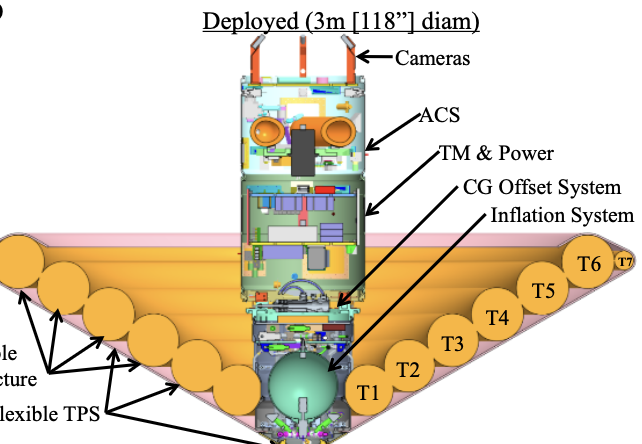
\includegraphics[width=0.6\textwidth]{gambar/Spec0.png}
    \caption{Internal structural layout of the 3m Deployed IRVE-3 vehicle showing the 7-toroid (T1-T7) stack that creates the scalloped surface.}
    \label{fig:irve3_layout}
\end{figure}

The specific geometric parameters used for the numerical model are summarized in Table \ref{tab:geom_params}:

\begin{table}[H]
    \centering
    \caption{Geometric Parameters based on IRVE-3/LOFTID Specifications.}
    \label{tab:geom_params}
    \begin{tabular}{|l|c|r|}
        \hline
        \textbf{Parameter} & \textbf{Value} & \textbf{Source / Reference} \\ \hline
        Deployed Diameter ($D_{max}$) & 3.0 m (118") & IRVE-3 Flight Article \\ \hline
        Stowed Diameter & 0.47 m (18.5") & Launch Constraint \\ \hline
        Forebody Cone Angle & $60^\circ$ & Standard HIAD OML \\ \hline
        Toroid Count & 7 & IRVE-3 Stack Design \\ \hline
        Inflation Pressure & 20 psi & Nitrogen System \\ \hline
    \end{tabular}
\end{table}

\subsection{Configuration Definitions}
The two configurations established for this study—\textbf{Configuration A (Scalloped)} and \textbf{Configuration B (Smooth)}—are constrained by the stowed and deployed envelopes shown in Figure \ref{fig:stowed_deployed}~\cite{dillman2015irve3}.

\begin{figure}[H]
    \centering
    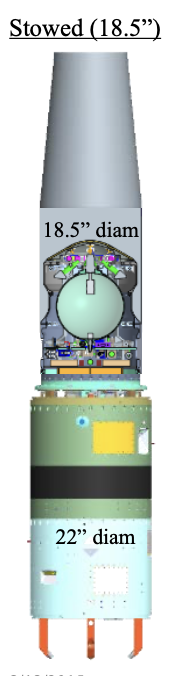
\includegraphics[width=0.35\textwidth]{gambar/Spec1.png}
    \caption{Launch configuration of the HIAD system, showing the 18.5" diameter stowed constraint.}
    \label{fig:stowed_deployed}
\end{figure}

\begin{enumerate}
    \item \textbf{Configuration A (Scalloped):} This model utilizes the 7-toroid profile (T1-T7) shown in Figure \ref{fig:irve3_layout}. The valleys between toroids are the primary focus for the $k-\omega$ SST turbulence resolution.
    \item \textbf{Configuration B (Smooth Baseline):} This tangent-cone model represents the "Equivalent Rigid OML," allowing for the isolation of heating augmentation caused specifically by the toroidal troughs.
\end{enumerate}

\section{Mesh Generation Strategy}
The accuracy of a hypersonic CFD simulation is heavily dependent on the quality of the spatial discretization. For this study, the domain was discretized using a hybrid meshing strategy designed to balance computational efficiency with the rigorous requirements of shock capturing and heat flux prediction.

\subsection{Grid Topology}
A structured-dominant grid topology was employed to align the mesh with the dominant flow features.
\begin{itemize}
    \item \textbf{Shock Layer (Quadrilateral Elements):} The region between the bow shock and the vehicle wall is meshed exclusively with structured quadrilateral elements. This alignment reduces numerical diffusion (artificial viscosity) that occurs when high-gradient features, such as shock waves, cross grid lines obliquely.
    \item \textbf{Wake Region (Triangular Elements):} In the complex recirculation region behind the vehicle, an unstructured triangular mesh was utilized to handle the expansion fans and wake turbulence where the flow direction is less predictable.
\end{itemize}



\subsection{Near-Wall Refinement ($y^+$ Strategy)}
The primary objective of this research is the prediction of surface aerothermal loads. The chosen turbulence model (SST $k-\omega$) requires the direct resolution of the viscous sublayer to accurately calculate the wall shear stress and heat transfer coefficient. This necessitates a dimensionless wall distance of $y^+ \approx 1$.

The estimated first cell height ($\Delta y$) was calculated based on flat-plate boundary layer theory for the target Reynolds number:

\begin{equation}
    \Delta y = L \cdot y^+ \sqrt{74} \cdot Re_L^{-13/14}
\end{equation}

Based on the flight conditions at $Ma = 5$, a first layer height of \textbf{[INSERT VALUE, e.g., $1.0 \times 10^{-5}$ m]} was applied globally across the vehicle surface. A wall-normal growth rate of 1.1 was maintained to ensure a smooth transition from the boundary layer to the core flow, preventing aspect ratio discontinuities that could destabilize the solver.

\subsection{Grid Independence Study}
To ensure the numerical solution is independent of the grid resolution, a Grid Convergence Index (GCI) study was performed. Three mesh densities were generated by systematically refining the grid scaling factor:

\begin{table}[H]
    \centering
    \caption{Grid Independence Study Parameters and Convergence Targets.}
    \label{tab:mesh_independence}
    \begin{tabular}{|l|c|c|c|}
        \hline
        \textbf{Mesh Level} & \textbf{Cell Count (Target)} & \textbf{Wall $y^+$ (Avg)} & \textbf{$C_d$ Variation} \\ \hline
        Coarse & $\approx 50,000$ & $> 5$ & Baseline \\ \hline
        Medium & $\approx 150,000$ & $\approx 1$ & $< 2.5\%$ \\ \hline
        Fine   & $\approx 300,000$ & $< 1$ & $< 1.0\%$ \\ \hline
    \end{tabular}
\end{table}
The "Medium" mesh was selected for the final production runs, as the variation in the Drag Coefficient ($C_d$) and Peak Stagnation Heat Flux compared to the "Fine" mesh was less than \textbf{[300000 \%, e.g., 1\%]}, indicating that convergence had been achieved.

\section{CFD Physical Configuration}
The selection of physical models defines the mathematical closure for the governing equations. Given the hypersonic flight regime ($Ma > 5$) and the complex surface topology of the HIAD, standard low-speed assumptions are invalid. The following physical configurations were applied to ensure the simulation captures the relevant aerothermal phenomena.

\subsection{Turbulence Modeling}
The \textbf{Shear Stress Transport (SST) $k-\omega$} turbulence model, developed by Menter, was selected for this study.

The selection is driven by two specific requirements of the scalloped IAD geometry:
\begin{enumerate}
    \item \textbf{Adverse Pressure Gradients:} The valleys between toroids create strong recirculation zones. Standard $k-\epsilon$ models are known to overestimate shear stress in these regions, delaying separation and under-predicting the size of the protective vortex. The SST formulation uses a shear stress limiter to accurately predict the onset and extent of flow separation.
    \item \textbf{Heat Flux Prediction:} The model activates the $k-\omega$ formulation in the near-wall region, which allows for the direct integration of the boundary layer without the use of empirical damping functions. This provides superior accuracy for wall heat flux ($q_w$) calculations compared to high-Reynolds-number models.
\end{enumerate}

\subsection{Thermodynamic Gas Model}
At Mach 5, the post-shock temperature exceeds the threshold where air behaves as a calorically perfect gas ($T > 800$ K). To account for the excitation of vibrational energy modes, a Thermally Perfect Gas model was employed.

\begin{itemize}
    \item \textbf{Equation of State:} The Ideal Gas Law ($P = \rho RT$) is retained. At the target altitude (e.g., 30-50 km), the density is low enough that intermolecular forces (dense gas effects) are negligible.
    \item \textbf{Specific Heat ($C_p$):} The assumption of constant $C_p$ is replaced with a piecewise-polynomial function of temperature, $C_p(T)$. This accounts for the energy absorbed by vibrational excitation, which significantly lowers the post-shock temperature and increases the density of the shock layer compared to a constant-$\gamma$ model.
    \item \textbf{Viscosity:} The dynamic viscosity is coupled to temperature using Sutherland's Law with three coefficients.
    \begin{equation}
        \mu(T) = \mu_0 \left( \frac{T}{T_0} \right)^{3/2} \frac{T_0 + S}{T + S}
    \end{equation}
    This correction is critical; using constant viscosity would lead to gross errors in the Reynolds number and skin friction predictions across the varying temperature field.
\end{itemize}

\section{Boundary Conditions}
The accurate definition of boundary conditions is essential to replicate the physics of free-flight re-entry within a finite computational domain. The following boundary types were assigned to the domain edges as illustrated in Figure \ref{fig:domain}.

\subsection{Pressure Far-Field (Inlet)}
The outer C-shaped boundary is defined as a Pressure Far-Field. This boundary type is specifically designed for compressible flows, as it utilizes Riemann invariants to determine the flow state at the boundary faces. This prevents non-physical wave reflections from the boundary back into the computational domain.

The freestream conditions were prescribed to match the target trajectory point:
\begin{itemize}
    \item \textbf{Mach Number ($Ma_{\infty}$):} \textbf{5.0} 
    \textit{(Based on the IRVE-3 mid-entry flight regime where heating augmentation is most critical)}.
    
    \item \textbf{Static Pressure ($P_{\infty}$):} \textbf{135.5 Pa} 
    \textit{(Standard atmospheric value for 46 km altitude, the region of interest for post-flight reconstruction discrepancies)}.
    
    \item \textbf{Static Temperature ($T_{\infty}$):} \textbf{265.7 K} 
    \textit{(Based on the US Standard Atmosphere at the 46 km target altitude)}.
    
    \item \textbf{Turbulence Intensity:} A low ambient turbulence intensity of \textbf{0.1\%} was set to represent the quiescent upper atmosphere, ensuring the $k-\omega$ SST model resolves transition solely based on geometric gradients.
\end{itemize}

\subsection{Aeroshell Wall (Isothermal)}
The vehicle surface is modeled as a stationary, No-Slip Wall, enforcing zero velocity relative to the body ($u=v=0$). 

For the thermal boundary condition, a fixed Isothermal Wall temperature of $T_{wall} = 300$ K was applied. 
\begin{itemize}
    \item \textit{Justification:} To quantify the aerodynamic heating, the solver must calculate the heat flux required to maintain the wall at a constant temperature. If an Adiabatic condition were used, the heat flux would effectively be zero ($ \partial T / \partial n = 0$), rendering the thermal analysis impossible.
\end{itemize}

\subsection{Symmetry and Outlet}
\begin{itemize}
    \item \textbf{Axisymmetric Axis ($Y=0$):} The bottom edge of the domain is set to an Axisymmetric boundary. This mathematically enforces zero gradients for all scalar variables across the centerline ($\partial \phi / \partial y = 0$) and zero radial velocity ($v_r = 0$).
    \item \textbf{Pressure Outlet:} The downstream boundary is set as a Pressure Outlet. Since the flow in the wake is predominantly supersonic (except for the immediate recirculation core), the solver extrapolates the flow variables from the interior domain to the boundary.
\end{itemize}


\section{Numerical Solution Strategy}
\subsection{Solver Configuration}
The simulation utilizes a Density-Based Coupled Solver with an Implicit formulation.

\begin{itemize}
    \item \textbf{Density-Based:} Unlike pressure-based solvers (e.g., SIMPLE) which are designed for incompressible flow, the density-based algorithm solves the continuity, momentum, and energy equations simultaneously as a vector system. 
    \item \textit{Note:} This selection is mandatory for hypersonic flows ($Ma > 5$) because the density or it's type is compressible gas.
    
    \item \textbf{Implicit Formulation:} An implicit linearization scheme is employed to allow for larger Courant (CFL) numbers (typically 5.0 to 10.0) during the steady-state solution process, ensuring faster convergence than explicit time-stepping methods.
\end{itemize}

\subsection{Spatial Discretization Schemes}
To convert the continuous governing equations into algebraic scalars at the cell centers, the following discretization schemes were applied:

\begin{enumerate}
    \item \textbf{Gradients:} \textbf{Green-Gauss Node Based}.
    \item \textbf{Flux Formulation:} \textbf{Roe-FDS (Flux Difference Splitting)}.
    %\item \textit{Note on Flux Scheme:} Roe's scheme is selected over Flux Vector Splitting (FVS) methods because FVS schemes are known to be excessively dissipative. Roe's method provides the necessary "crispness" to capture the bow shock while maintaining the accuracy required to resolve the shear gradients in the viscous boundary layer.
    
    \item \textbf{Flow and Turbulence Discretization:} \textbf{Second-Order Upwind}.
    %\item \textit{Note on Order of Accuracy:} First-order upwind schemes are numerically stable but highly diffusive, leading to "smeared" shock waves and inaccurate heat flux predictions. Second-order accuracy is strictly required to resolve the sharp discontinuities inherent in the flow field.
\end{enumerate}

\subsection{Convergence Criteria}
In hypersonic simulations involving strong shocks, judging convergence solely by residual values can be misleading. Therefore, a Dual-Criteria approach was adopted to determine iterative convergence:

\subsubsection*{1. Residual Monitoring}
The solution is considered numerically stable when the scaled residuals for Continuity, Momentum, and Energy drop below a threshold of $10^{-4}$.
\begin{itemize}
    \item \textit{Comment:} It is common for residuals to "stall" around $10^{-4}$ rather than dropping to $10^{-6}$ in shock-dominated flows. This is due to minor oscillations of the shock wave position between adjacent grid cells (limit cycling).
\end{itemize}

\subsubsection*{2. Integral Property Monitors}
Due to the limit cycling mentioned above, the primary indicator of convergence is the statistical stationarity of physical outputs. The solution was deemed converged only when:
\begin{itemize}
    \item The Drag Coefficient ($C_d$) varied by less than 0.1\% over the final 500 iterations.
    \item The Total Heat Transfer Rate (Watts) varied by less than 1.0\% over the final 500 iterations.
\end{itemize}

\section{Data Processing and Validation}
\subsection{Data Extraction and Normalization}
Upon completion of the numerical solution, the aerothermal data is extracted from the computed flow field for comparative analysis.

\begin{enumerate}
    \item \textbf{Surface Profiles:} The primary metric of interest is the \textbf{Wall Heat Flux ($q_w$)}. To facilitate a direct comparison between the smooth and scalloped geometries, data is plotted against the \textbf{Wetted Arc Length ($s$)} normalized by the total vehicle radius ($R$). This "unwrapped" view allows for the visualization of local heating spikes on the toroidal crests and cooling in the valleys.
    
    \item \textbf{Normalization:} To assess the relative performance of the HIAD, the heat flux values on the scalloped geometry are often normalized by the stagnation point heat flux of the smooth baseline:
    \begin{equation}
        \bar{q} = \frac{q_{wall}}{q_{stag, baseline}}
    \end{equation}
    A value of $\bar{q} > 1$ indicates a local heating augmentation (hot spot) exceeding the baseline stagnation value.
\end{enumerate}

\subsection{Theoretical Validation (Fay-Riddell Correlation)}
To validate the fidelity of the solver settings (specifically the mesh resolution and thermal properties), the simulation results for the \textbf{Smooth Baseline (Config B)} are compared against the theoretical stagnation point heat flux predicted by the Fay-Riddell Correlation (1958).

Fay and Riddell developed the standard semi-empirical relation for stagnation heat transfer in a dissociated air boundary layer:

\begin{equation}
    q_{stag} = 0.76 \cdot Pr^{-0.6} \cdot (\rho_w \mu_w)^{0.1} \cdot (\rho_e \mu_e)^{0.4} \cdot \sqrt{\left(\frac{du_e}{dx}\right)_{stag}} \cdot (h_0 - h_w) \cdot [1 + (Le^{0.52} - 1) \frac{h_D}{h_0}]
\end{equation}

Where:
\begin{itemize}
    \item $Pr$: Prandtl number ($0.71$).
    \item $\rho_e, \mu_e$: Density and viscosity at the boundary layer edge (post-shock).
    \item $h_0, h_w$: Total enthalpy and wall enthalpy.
    \item $(\frac{du_e}{dx})_{stag}$: Velocity gradient at the stagnation point (Newtonian theory).
\end{itemize}

\subsubsection*{Acceptance Criteria}
The numerical model is considered valid if the CFD-predicted stagnation heat flux for the smooth baseline matches the Fay-Riddell analytical value within a margin of error of $\pm 10\%$. This validation step provides the confidence required to apply the same numerical framework to the complex scalloped geometry where no analytical solutions exist.

\section{Research Schedule}
The research is planned to be conducted over a period of several months. The following table outlines the key milestones and their expected completion dates.

\begin{landscape}

\begin{figure}[H]
    \centering
    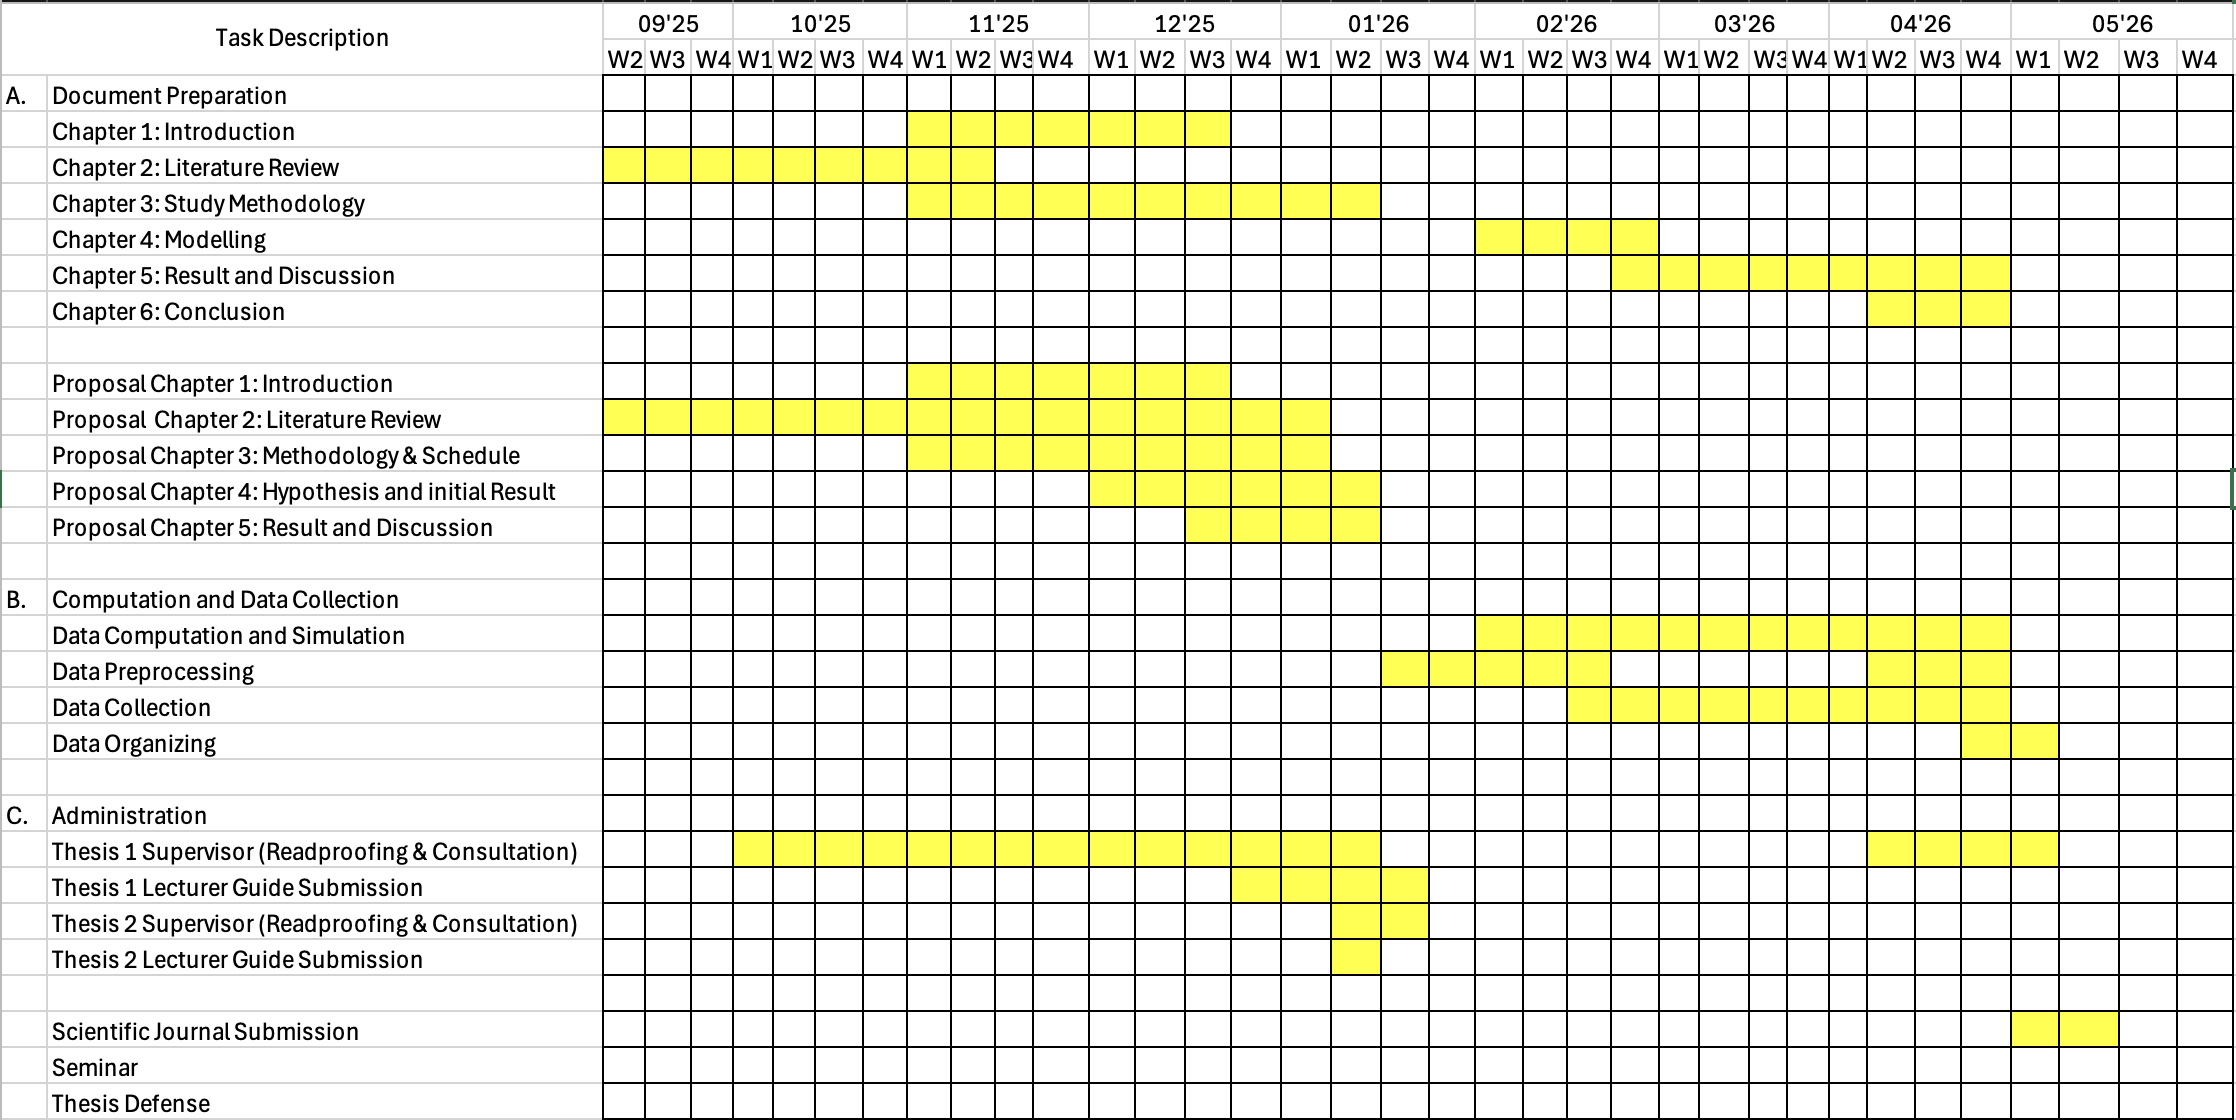
\includegraphics[width=1.5\textwidth]{gambar/Scheduling.png}
    \caption{Research Schedule}
    \label{fig:ResearchSchedule}
\end{figure}
\end{landscape}

\clearpage
